\section{Main results}\label{sec_main}

In case (i), we provide the exact asymptotics for both the bias and variance terms, together with almost sharp convergence rates. We will use these results to illustrate the effects of the \emph{bias-variance tradeoff} and \emph{varying sample sizes}. In case (ii), we will prove an exact asymptotic variance limit, and employ the result to show the intricate effect of the covariate shift. On the other hand, in case (ii), we will provide an estimate on the bias term, which becomes exact only when $n_1\gg p$. 


\subsection{Covariate shift}\label{sec_diff}

We begin by considering the covariate shift setting where both tasks have the same linear model but different population covariance matrices.
We show the exact asymptotic limit of the excess risk of the HPS estimator in the high-dimensional setting.

First, we consider the variance. Recall from equation \eqref{Lvar} that the variance equation is equal to $\sigma^2 \cdot \bigtr{\Sigma^{(2)} (\hat\Sigma(a))^{-1}}$.
In particular, the matrix $\hat{\Sigma}$ adds up both tasks' sample covariance matrices.
Thus, the expectation of $\hat{\Sigma}(a)$ is equal to a mixture of both tasks' population covariance matrices, with mixing proportions determined by their sample sizes.
Intuitively, the spectrum of $\hat{\Sigma}(a)^{-1}$ now not only depends on the sample sizes of both tasks, but also depends on how well ``aligned'' $\Sigma^{(1)}$ and $\Sigma^{(2)}$ are.
To capture this alignment quantitatively, we introduce the covariate shift matrix %(rescaled by $a$)
$$ M \define (\Sigma^{(1)})^{\frac 1 2}(\Sigma^{(2)})^{-\frac 1 2}.$$
Let $\lambda_1 \ge \lambda_2 \ge \dots\ge \lambda_p $ be the singular values of $M$ in descending order.
Our first main result is the following theorem on the variance limit, which characterizes the exact dependence of $L_{\var}(a)$ on the singular values of $M$.


\begin{theorem}[Variance estimates under covariate shift]\label{thm_main_RMT}
Under Assumption \ref{assm_big1} (recalling $\varphi > 4$), for any small constant $c>0$, there exists a high probability event $\Xi$, on which the following estimate holds for $L_{\var}(a)$ in \eqref{Lvar}:
	\begin{align}\label{lem_cov_shift_eq}
		\bigabs{L_{\var}(a)- \frac{\sigma^2}{n_1+n_2}\bigtr{  \frac{1}{\alpha_1 a^2\cdot M^\top M + \alpha_2}  }}
		\le \frac{(n_1+n_2)^{\frac 2{\varphi} - \frac 1 2 + c}}{p^{1/2}}\cdot\frac{p \sigma^2}{n_1+ n_2},
	\end{align}
	uniformly in all $a\in \R$. Here $(\alpha_1, \alpha_2)$ is the solution of the following system of equations
	\begin{align}
		\alpha_1 + \alpha_2 = 1- \frac{p}{n_1 + n_2}, \quad
		\alpha_1 + \frac1{n_1 + n_2}  \bigbrace{\sum_{i=1}^p \frac{(a \lambda_i)^2 \alpha_1}{(a \lambda_i)^2 \alpha_1 + \alpha_2}} = \frac{n_1}{n_1 + n_2}. \label{eq_a12extra}
	\end{align}
\end{theorem}
\todo{changed $a_1, a_2$ to $\alpha_1, \alpha_2$ since they conflict with $a$}

Equation \eqref{lem_cov_shift_eq} thus characterizes the variance of the HPS estimator, up to an error term on the order of $O\big(\frac{\sigma^2}{p^{-1/2}}\big)$ (recall that $\varphi > 4$, $c$ is an arbitrarily small constant, $\frac{p}{n_1+n_2} \in (2 {\tau}, \frac 2 {\tau})$).
Our result can be viewed as a generalization of the classical result in Lemma \ref{fact_tr} to the \textit{covariate shift} setting.
In particular, Lemma \ref{fact_tr} corresponds to a setting where the singular values $\lambda_1,\dots,\lambda_p$ are all equal to one, and $a = 1$. Then, the second part of equation \eqref{eq_a12extra} simplifies to
\[ \alpha_1 + \frac{p}{n_1 + n_2}\cdot \frac{\alpha_1}{\alpha_1 + \alpha_2} = \frac{n_1}{n_1 + n_2}. \]
By solving the above together with the first part of equation \eqref{eq_a12extra}, we obtain that
$$\alpha_1 = \frac{n_1}{n_1+n_2},\quad \alpha_2 = \frac{n_2-p}{n_1+ n_2}.$$
Plugging the above solutions back to the variance limit, we thus find that the limit is equal to
\begin{align}
    \frac{\sigma^2}{n_1 + n_2} \bigtr{\frac 1 {\alpha_1 M^{\top} M + \alpha_2}} &= \frac{\sigma^2}{n_1 + n_2} \frac{p}{\alpha_1 + \alpha_2} \tag{since the singular values of $M$ are equal to $1$} \nonumber \\
    &= \frac{\sigma^2}{n_1 + n_2} \cdot\frac{p (n_1 + n_2)}{n_1 + n_2 - p} \tag{applying $\alpha_1$ and $\alpha_2$ from above} \nonumber \\
    &= \frac{\sigma^2 p}{n_1 + n_2 - p}, \label{g_id}
\end{align}
which is precisely the limit in Lemma \ref{fact_tr}.
Additionally, the convergence rate in equation \eqref{lem_cov_shift_eq} matches the one in Lemma \ref{fact_tr} for this special case.
%With Assumption \ref{assm_big1},
%$$ \frac{\sigma^2}{n_1+n_2}\bigtr{  \frac{1}{a_1 M(a)^\top M(a) + a_2  }  } \sim \frac{p \sigma^2}{n_1+ n_2}.$$
%Hence the right-hand side of \eqref{lem_cov_shift_eq} is much smaller than this main term by a factor of $p^{-1/2} (n_1+n_2)^{-1/2+2/\varphi + c}$, which we believe to be sharp up to the $(n_1+n_2)^c$ factor. Lemma \ref{fact_tr} can be also regarded as a special case of Theorem \ref{thm_main_RMT}. %also extends  to the inverse of the sum of two sample covariance matrices.
The proof of Theorem \ref{thm_main_RMT}, which is based on recent developments in random matrix theory \cite{Anisotropic}, can be found in Section \ref{appendix RMT}.

Second, we consider the bias.
Note that the setting where $\beta_1 = \beta_2$ can be viewed as a special case of the random-effect model with $d = 0$, thus, assuming that $\norm{\beta_1}_2^2 \ge \sigma^2 / p^{1/2 - c_0}$ for a small constant $c_0 > 0$, we have that $\hat B_1 / \hat B_2$ is equal to $1$ plus lower-order terms that scale to zero as $p$ goes to infinity (see equation \eqref{hatw_add1} for the precise scaling).
In Proposition \ref{lem_hat_v}, we have seen that the global minimizer $\hat a$ is close to 1 up to a small error.
Thus, the bias equation $L_{\bias}(\hat B_1 / \hat B_2)$ is equal to $0$ plus the above lower-order terms.
We summarize this discussion in the following corollary:

\begin{corollary}[Excess risk of HPS under covariate shift]\label{cor_hps_cov}
    Under Assumption \ref{assm_big1}, suppose further that $\beta_1 = \beta_2$ and $\norm{\beta_1}^2_2 \ge \frac{\sigma^2}{p^{1/2 - c_0}}$ for a constant $c_0 > 0$.
    Then, for any constant $c > 0$, the following estimate on the excess risk of the HPS estimator holds w.h.p.
    \begin{align}
        \bigabs{L(\hat{\beta}_2^{\MTL}) - \frac{\sigma^2}{n_1 + n_2} \bigtr{\frac{1}{\alpha_1 M^{\top} M + \alpha_2}}}
        \le
        \OO\bigbrace{\frac{(n_1+n_2)^{\frac 2{\varphi} - \frac 1 2 + c}}{p^{1/2}}\cdot\frac{p \sigma^2}{n_1+ n_2}
        + p^{-c_0 + 2c}},
    \end{align}
    where $\alpha_1$ and $\alpha_2$ are the solutions of equation \eqref{eq_a12extra} after taking $a = 1$.
\end{corollary}


\begin{figure}[!t]
	\begin{subfigure}[b]{0.5\textwidth}
		\centering
		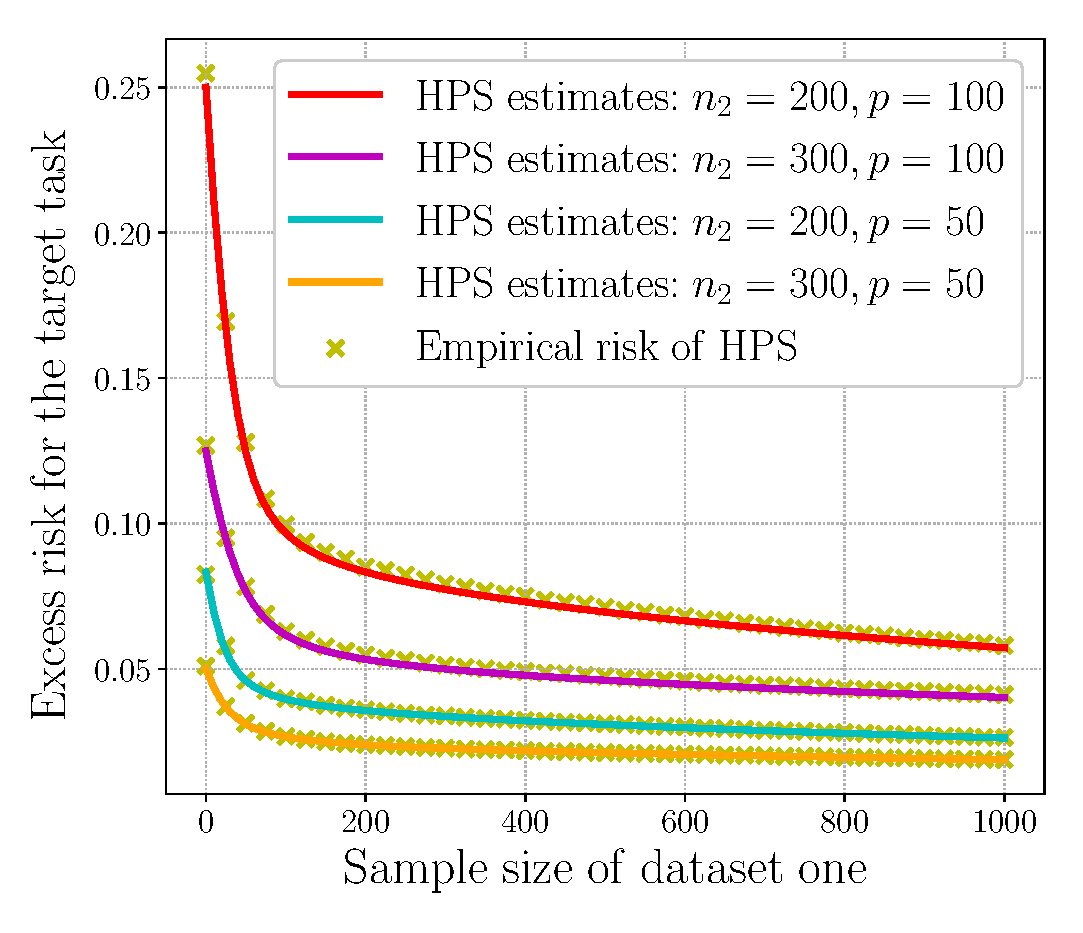
\includegraphics[width=0.8\textwidth]{figures/verify_covariate_shift.eps}
		\caption{Illustrating variance estimates for finite $p$}
		\label{fig_sec3_verify_cov}
	\end{subfigure}
	\begin{subfigure}[b]{0.5\textwidth}
		\centering
		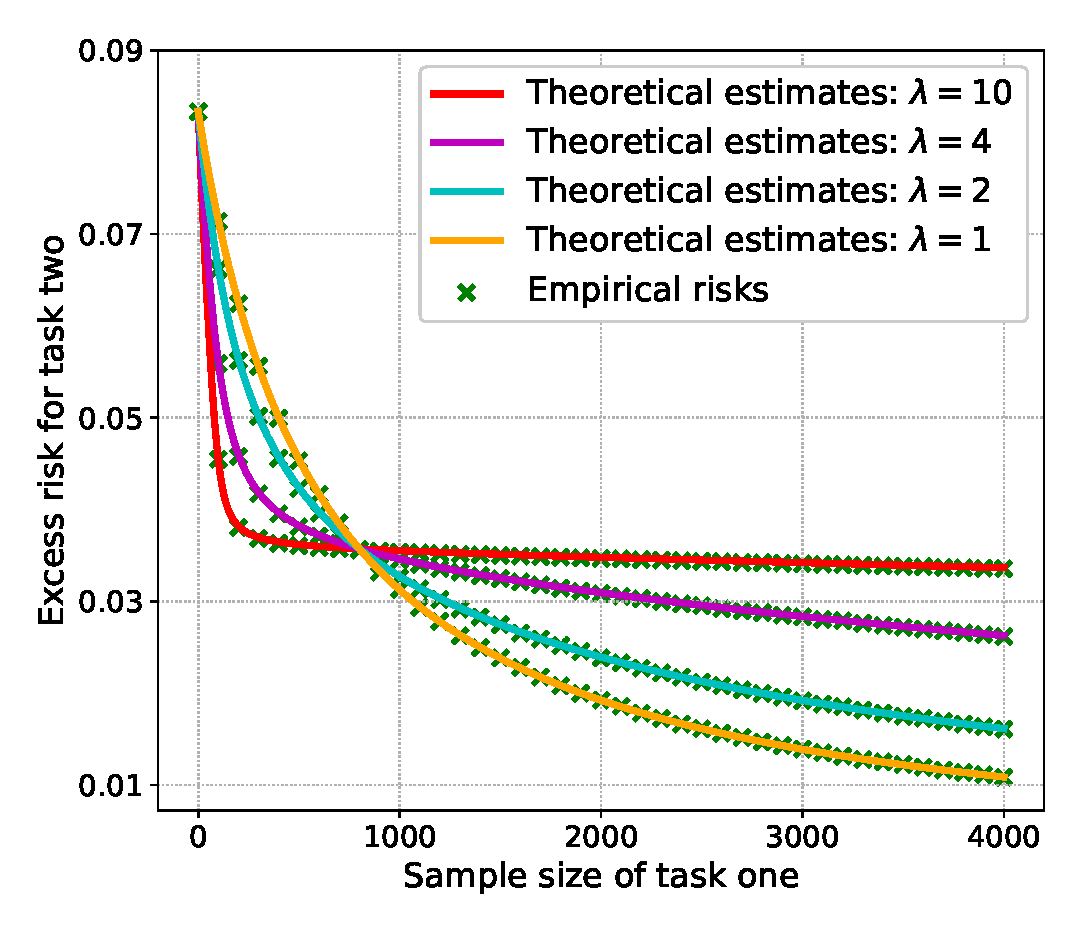
\includegraphics[width=0.8\textwidth]{figures/covariate_shift.eps}
		\caption{Sample sizes vs. covariate shift}
		\label{fig_sec3_covariate}
	\end{subfigure}
	\caption{We verify that Theorem \ref{thm_main_RMT} provides incredibly accurate estimates of the empirical variance under various finite sample sizes and dimensions.
	Furthermore, we illustrate an intriguing dichotomy between sample sizes and covariate (cf. Claim \ref{claim_dichotomy}).
	When $n_1 \ge n_2$, the lowest risk for predicting task two's labels is achieved by transferring from a dataset that has the same covariance matrix as task two. 
	When $n_1 < n_2$, the lowest risk is instead achieved by transferring a covariate-shifted dataset.
	Both simulation uses $\sigma = 1/2$.
	Figure \ref{fig_sec3_verify_cov} fixes $\lambda = 4$ and varies $n_1, p$.
	Figure \ref{fig_sec3_covariate} fixes $p = 100, n_2 = 300$ while varying $n_1, \lambda$.}
	\label{fig_sec31}
\end{figure}

\paragraph{Illustrative examples.} Next, we illustrate the result of Corollary \ref{cor_hps_cov} in several examples.
We use our estimates to explore whether covariate shift helps or hurts information transfer.
Our first example illustrates that the effect of covariate shift depends on the sample sizes of each dataset in an intricate manner.
    While the folklore belief is that transferring from a covariate-shifted distribution performs worse than an identical distribution, we show that, surprisingly, the former can sometimes outperform the latter.
    
    We first describe a setting for modeling covariate shift.
    Let $\cS$ be the set of positive definite matrices $M^{\top} M$ such that for $i = 1,2,\dots,\floor{\frac p 2}$, $\lambda_{p - i}  = \frac 1 {\lambda_i}$, where $\lambda_1 \ge \lambda_2 \ge \cdots \ge \lambda_p$ are the eigenvalues of $M$.
    Under this setting, we ask: suppose that the sample sizes $n_1$ and $n_2$ are both fixed, which $M$ provides the best ``transfer'' in the sense of HPS estimator's excess risk?
    We observe a dichotomy that depends on whether or not $n_1$ is greater than $n_2$.
    \begin{claim}[Sample sizes vs. covariate shift]\label{claim_dichotomy}
        Let $g(M) = \frac{\sigma^2}{n_1 + n_2} \bigtr{\frac 1 {\alpha_1 M^{\top} M + \alpha_2}}$.
        Suppose that $n_1$ and $n_2$ are both fixed.
        Within the set of all possible covariate shift matrix $M\in\cS$, the following dichotomy holds:
        \begin{enumerate}
	        \item[i)] If $n_1 \ge n_2$, then $g(M)$ is minimized in $\cS$ when $\lambda_i = 1$, for any $i = 1,\dots,p$.
	        \item[ii)] If $n_1 < n_2$, then $g(M)$ is maximized in $\cS$ when $\lambda_i = 1$, for any $i = 1,\dots,p$.
        \end{enumerate}
    \end{claim}

\begin{proof}
    For any $M \in \cS$, we can write $g(M)$ as
    $$g(M)=\frac{\sigma^2}{ n_1+n_2 }\sum_{i=1}^{p/2}\left( \frac{1}{\lambda_i^{2} \alpha_1 + \alpha_2} + \frac1{\lambda_i^{-2} \alpha_1 + \alpha_2} \right).$$
    When $M=\id_{p\times p}$, by the first equation of \eqref{eq_a12extra}, we have
    $$g(\id_{p\times p})=\frac{\sigma^2}{ n_1+n_2 }\sum_{i=1}^{p/2} \frac{2}{1-\gamma},$$
    where we abbreviate $\gamma:=p/(n_1+n_2)$.
    Using $\alpha_1 + \alpha_2 = 1-\gamma$, we further have that
    \begin{align*}
        g(M) - g(\id_{p\times p})%&= \frac{\sigma^2 \gamma}{2(1-\gamma)} (\lambda^2-1)a_1\cdot \bigbrace{  \frac{1}{ -a_1(\lambda^2-1)+(1-\gamma)\lambda^2 } - \frac{1}{a_1(\lambda^2-1) + (1-\gamma)}} \\
        &= \frac{\sigma^2 }{ n_1+n_2-p} \sum_{i=1}^{p/2} \frac{(\lambda_i^2-1)^2 \alpha_1 \left[ \alpha_1 - \alpha_2\right] }{[\alpha_1 + \lambda_i^2 \alpha_2][\lambda_i^2 \alpha_1 + \alpha_2]} .
    \end{align*}
    %in this example is equal to
    %$\frac{p}{2(n_1 + n_2)} f(\lambda)$, where
    %\[ f(\lambda) = {(\lambda^{-2} a_1 + a_2)^{-1} + (\lambda^2 a_1 + a_2)^{-1}}. \]
    %Using the fact that $a_1 + a_2 = 1 - \frac{p}{n_1 + n_2}$, we can verify
    %\begin{align*}
    %	f(\lambda) - f(1) &= \left(\lambda^2 a_1 + \frac{n_1 + n_2 - p}{n_1 + n_2} - a_1\right)^{-1} \\
    %	&+ \left(\lambda^{-2} a_1 + \frac{n_1 + n_2 - p}{n_1 + n_2} - a_1\right)^{-1} \\
    %	&- \frac{2(n_1 + n_2)}{n_1 + n_2 - p} \\
    %	&= \left(2a_1 - \frac{n_1 + n_2-p} {n_1 + n_2 }\right)  g(\lambda, a_1), %\cdot (\lambda^2-1)^2
    %\end{align*}
    %\begin{align*}
    %	f(\lambda) - f(1) &= \left(2a_1 - \frac{n_1 + n_2-p} {n_1 + n_2 }\right)  g(\lambda, a_1), %\cdot (\lambda^2-1)^2
    %\end{align*}
    %where $g(\lambda, a_1) \ge 0$.
    %and can be derived from algebraic calculations (details omitted).
    We claim that $\alpha_1 > \alpha_2$ if and only if $n_1 > n_2$, which proves claim i).
    In fact, if $\alpha_1 > \alpha_2$, then the first part of equation \eqref{eq_a12extra} gives that $\alpha_1 > (1-\gamma)/2$.
    The second part of equation \eqref{eq_a12extra} gives that
    \begin{align*}
     \frac{n_1}{n_1 + n_2} &> \alpha_1 + \frac{1}{n_1+n_2} \sum_{i=1}^{p/2}\left(\frac{\lambda_i^2}{\lambda_i^2+1}+\frac{\lambda_i^{-2}}{\lambda_i^{-2}+1}\right) = \frac{1-\gamma}{2}+\frac{\gamma}{2}=\frac{1}{2},
    \end{align*}
    %\begin{align*}
    % \frac{n_1}{n_1 + n_2} &=a_1 + \frac1{n_1 + n_2}\cdot \bigbrace{\sum_{i=1}^p \frac{\lambda_i^2 a_1}{\lambda_i^2 a_1 + a_2}} \\
    %	&> a_1 + \frac{p}{2(n_1+n_2)} \left(\frac{\lambda^2}{\lambda^2+1}+\frac{\lambda^{-2}}{\lambda^{-2}+1}\right) =\frac{1}{2}.
    %\end{align*}
    which is equivalent to $n_1>n_2$. The proof of claim ii) follows from a similar argument. % Similarly, if $a_1<a_2$, equations  \eqref{eq_a12extra000} and  \eqref{eq_a12extra} give that $a_1 < \frac{n_1 + n_2-p}{2 (n_1 + n_2)}$ and $n_1<n_2$. Thus, we conclude that $f(\lambda) \ge f(1)$ if and only if $n_1 \ge n_2$.
    %\end{example}
\end{proof}

Figure \ref{fig_sec3_covariate} illustrates a special case where $\lambda_1 = \cdots = \lambda_{\floor{p /2}} = \lambda > 0$ and the rest of the eigenvalues are all equal to $1 / \lambda$.
Thus, $\lambda > 0$ captures the degree of covariate shift: higher $\lambda$ implies worse covariate shift.
We observe that our theoretical estimates using Corollary \ref{cor_hps_cov} matches the empirical risks incredibly accurately.
As a result, we indeed observe the dichotomy shown in Claim \ref{claim_dichotomy}.
Furthermore, for higher $\lambda$, HPS' excess risk decreases slower--indicating a worse rate of ``transfer'' from task one. 
As a remark, the classical work of \citet{david2010impossibility} have likewise shown impossibility results for transfer learning under covariate shift in a classification setting.
By contrast, our analysis applies to a (high-dimensional) regression setting.


Our second example illustrates that the effect of covariate shift worsens as the sample size of task one increases.
We consider a set of covariate shift matrices $M^{\top} M$ whose determinant are all equal to one, and the eigenvalues are bounded between $\tau^2$ and $1 / \tau^2$.
Let $\cS$ denote the set of $M\in\real^{p\times p}$ such that $M^{\top} M$ satisfies both conditions.
\begin{claim}[Identical covariance provides approximately optimal transfer under imbalanced dataset sizes]\label{prop_covariate}
    Recall that $g(M) = \frac{\sigma^2}{n_1 + n_2} \bigtr{\frac 1 {\alpha_1 M^{\top} M + \alpha_2}}$.
	We have the following result regarding $g(\id_{p \times p})$:
	\begin{align} g(\id_{p\times p}) \le \bigbrace{1+ {\frac{n_2}{\tau^2 n_1}  }} g(M), \text{ for any } M \in \cS. \label{eq_claim_id}
	\end{align}
\end{claim}
\begin{proof}
    We can write down the trace of $(\alpha_1 M^{\top} M + \alpha_2)^{-1}$ using the eigenvalues of $M^{\top} M$ as follows:
    \begin{align*}
        (\alpha_1 M^{\top} M + \alpha_2)^{-1} &= \sum_{i=1}^p \frac{1} {\alpha_1 \lambda_i^2 + \alpha_2} \\
        &\ge \sum_{i=1}^p \frac{1} {\alpha_1 \lambda_i^2 + \alpha_2 \cdot {\lambda_i^2} / {\tau^2}} \tag{since $\lambda_i \ge \tau$, for any $i$} \\
        &= \frac 1 {\alpha_1 + \alpha_2 / \tau^2} \sum_{i=1}^ p \frac 1 {\lambda_i^2} \\
        &\ge \frac 1 {\alpha_1 + \alpha_2 /\tau^2} p\cdot \bigbrace{\prod_{i=1}^p \frac 1 {\lambda_i^2}}^{1/ p} \tag{by the AM-GM inequality} \\
        &= \frac{p}{\alpha_1 + \alpha_2 / \tau^2} \tag{since $\prod_{i=1}^p \lambda_i^2 = \det(M^{\top} M) = 1$}
    \end{align*}
    Next, recall from equation \eqref{g_id} that
    $g(\id_{p\times p}) = \frac{\sigma^2 p}{n_1 + n_2 - p}$.
    Thus, equation \eqref{eq_claim_id} follows if we show that (after rearranging terms)
    \begin{align}
        \frac{n_1 + n_2}{n_1 + n_2 - p} \cdot \frac 1 {\alpha_1 + \frac{\alpha_2}{\tau^2}} \le 1 + \frac{n_2}{\tau^2 \cdot n_1}. \label{eq_claim_id_step}
    \end{align}
    From the second part of equation \eqref{eq_a12extra}, we have that
    \begin{align*}
        \frac{n_1} {n_1 + n_2} &= \alpha_1 + \frac 1 {n_1 + n_2} \bigbrace{\sum_{i=1}^p \frac{\lambda_i^2\alpha_1}{\lambda_i^2\alpha_1 + \alpha_2}} \\
        &< \alpha_1 + \frac p {n_1 + n_2}.
    \end{align*}
    Thus, $\alpha_1 > \frac{n_1 - p}{n_1 + n_2}$, which implies that $\alpha_2 < \frac{n_2}{n_1 + n_2}$.
    Hence, $\alpha_1 + \frac{\alpha_2}{\tau^2} = 1 - \frac{p}{n_1 + n_2} - \alpha_2 + \frac{\alpha_2}{\tau^2} \le 1 - \frac{p}{n_1 + n_2} + \frac{n_2}{n_1 + n_2} \frac 1 {\tau^2}$, which implies
    equation \eqref{eq_claim_id_step} by straightforward calculations.
    Thus, the proof is complete.
\end{proof}
As a corollary of Claim \ref{prop_covariate}, when $n_1$ is much larger than $n_2 / \tau^2$, the excess risk of HPS is approximately optimal in the set of all possible $M\in\cS$ when there is no covariate shift between dataset one and two.





\subsection{Model shift}\label{sec_sizeratio}

Next, we consider a model shift setting where task one and two have the same linear model but different population covariance matrices.
We show the exact asymptotic limits of the bias and variance of HPS.

\begin{theorem}[Excess risk of HPS under model shift]\label{cor_MTL_loss}
Under Assumption \ref{assm_big1}, suppose that $\Sigma^{(1)}=\Sigma^{(2)}$ and the entries of $Z^{(1)}$ and $Z^{(2)}$ are i.i.d. Gaussian random variables.
Denote by $\xi_1:=p/n_1$ and $\xi_2:=p/n_2$.
Then, for any small constant $\e>0$ and large constant $C>0$, there exists a high probability event $\Xi$, on which the following estimates hold uniformly in all $a\in \R$:
\begin{align}
L_{\var}(a) &= \sigma^2  \cal L_1(a)+ \OO\Big(\frac {\sigma^2 p^{c}} {n_1}\Big), \label{Lvar_samplesize} \\
L_{\bias}(a)&= \bignorm{\beta^{(1)}-a\beta^{(2)}}^2 \cal L_2(a) +  \OO\Big(p^{-\frac 1 2 + c}  \norm{\beta^{(1)}-a\beta^{(2)}}^2
+ p^{-C}\big( \|\beta^{(1)} \|^2  +  \|\beta^{(2)} \|^2\big)   \Big),\label{Lbias_samplesize}
\end{align}
where $\cL_1(a)$ and $\cL_2(a)$ are defined as follows
\begin{align*}
\cal L_1(a) &:= {2p}\cdot\left((n_2 - p) + a^2 (n_1 - p) + \sqrt{\big( (n_2 - p) + a^2 (n_1 - p)\big)^2 + 4a^2(n_1 p + n_2 p - n_1 n_2)}\right)^{-1}, \\
\cal L_2(a) &:= \frac1{a^2}\cdot \frac{1- 2\frac{\cal L_1(a)}{\xi_2(1 + \cal L_1(a))} + \kappa(a)}{1- \xi_2 \kappa(a)}, \text{ in which }
\kappa(a) := \frac{\cal L_1(a)^2}{\xi_2^2(1+\cal L_1(a))^2}  \left(1 - \frac{a^4 \cal L_1(a)^2 }{\xi_1(1+a^2\cal L_1(a) )^2}\right)^{-1}.
%f_2(a):= \frac{a^4 \cal L_1(a)^2}{\xi_1^2 } \left[1 - \frac{a^4 \cal L_1(a)^2 }{\xi_1[1+a^2\cal L_1(a) ]^2}\right]^{-1},\\
%f_3(a):= \frac1{a^2}\frac{\xi_1}{\xi_2 +\cal L_1(a)}
 \end{align*}
%	In the setting of Example \ref{ex_sample_ratio}, assume that
%	%a) the sample sizes $n_1$ and $n_2$ are greater than $(1 + \tau) p$, b) $\Sigma_1=\Sigma_2=\id_p$, and c) %there exists a small constant $c_0>0$ such that
%	(i) both tasks sample sizes are at least $3p$;
%	(ii) noise variance is smaller than the shared signal variance: $\sigma^2 \lesssim  \kappa^2$;
%%	\be\label{choiceofpara0}
%%	p^{-1/2+c_0}\sigma^2 + p^{c_0}d^2\le \kappa^2\le p^{1-c_0} (\sigma^2 +d^2)  .  	\ee
%	%\be\label{choiceofpara0}
%%	(ii) the task-specific variance of $\beta_i$ is much smaller than the signal strength {\color{red}$d^2 = \oo( {\kappa^2})$}; \HZ{what does $\ll$ mean exactly?}
%%	(iii) the sample sizes $n_1$ and $n_2$ are greater than $(1 + \tau) p$.
%	(iii) task-specific variance is much smaller than the shared signal variance: $d^2 \le p^{-\e}{\kappa^2}$ for a small constant $c>0$.
%	Let $\varepsilon = (1 + \sqrt{p/n_1})^ 4 - 1$, which decreases as $n_1$ increases.
%	Let $\hat{A},\hat{B}$ be the global minimizer of $f(A, B)$.
%	With high probability over the randomness of the input,
%	the prediction loss of $\hat{\beta}_2^{\MTL} = \hat{B} \hat{A}_2$ for task two satisfies that
%	\begin{align}
%	%-\left[1- \left( 1-\frac{1}{\sqrt{\rho_1}}\right)^4\right] pd^2\cdot \frac{\rho_1^2 (\rho_1+\rho_2)}{(\rho_1 + \rho_2 - 1)^3} +\OO(p^{-c}\sigma^2)  \le
%	   \left|L(\hat{\beta}_2^{\MTL}) - \frac{2d^2 n_1^2 (n_1 + n_2)}{(n_1 + n_2 - p)^3} -\frac{\sigma^2 p}{n_1 + n_2 - p}  \right|
%	\le \varepsilon \cdot \frac{2d^2 n_1^2 (n_1 + n_2)}{(n_1 + n_2 - p)^3} +  \OO(p^{-c/2}).\label{cor_MTL_error}
%	%\left[\left( 1+\frac{1}{\sqrt{\rho_1}}\right)^4-1\right] d^2\cdot \frac{\rho_1^2 (\rho_1+\rho_2)}{(\rho_1 + \rho_2 - 1)^3} \\
%	%& +C \left[(p^{-c_\varphi}+p^{-c_\infty/2})(\sigma^2 +d^2)+p^{-c_\infty}\kappa^2 + %\frac{d^4+\sigma^2 d^2}{\kappa^2}\right],\nonumber
%	 \end{align}
%	 with high probability for any fixed $c\in(0, \min(\frac{1}{4}, \delta,\frac{\varphi-4}{2\varphi}))$.
%	 {\color{red}[FY: the error also contains $p^{-1/2+2c}\kappa^2 +  p^{-1/4+c} (\sigma^2 +d^2) $, both of which cannot be omitted, because (i) there is no assumption on the upper bound of $\kappa^2$, and (ii) we do not necessarily have $c_\varphi<1/4$. We can decide how to present the result concisely (for instance we can impose an upper bound on $\kappa^2$ and that $c_\varphi<1/4$), but it needs to be correct.]}
	 \end{theorem}

\iffalse
 We need to state a result for Gaussian matrix ...... Consider
$$f (\al,n_1,n_2)= \frac1p\tr\left[\frac{1}{ (X_1^\top X_1 + \al \cdot X_2^\top X_2)^2} (X_1^\top X_1)^2\right].$$
In our case, we have $\al=1$, but we can handle more general $\al$. We introduce two parameters:
$$a= \al \frac{n_2}{n_1} \left( \frac{p}{n_1} + \frac{p}{n_2}- \frac{p}{n_1 }\cdot \frac{p}{n_2}\right),\quad b= \al \frac{n_2}{n_1}\left( 1- \frac{p}{n_2}\right) + \left( 1- \frac{p}{n_1}\right). $$
Then we define the following parameters:
\begin{align*}
x= \frac{-b+ \sqrt{b^2 + 4a}}{2a},\quad y= \left[ x^{-2} - \frac{p}{n_1}\left( 1+\frac{p}{n_1}x\right)^{-2}\right]^{-1},\quad \omega= \al\frac{n_2}{n_1} \left( 1 + \al \frac{p}{n_1}x\right)^{-1}.
\end{align*}
We have that
$$f(\al,n_1,n_2)= \frac{1 - 2\omega x + \omega^2 y}{ 1 - \frac{p}{n_2} \cdot \omega^2 y } +\oo(1)\quad \text{w.h.p.} $$
In the setting $\al=1$, both $\omega x$ and $\omega^2 y$ can be written in terms of only one parameter
%$$f(\al,n_1,n_2)= \frac{\left(u^2 -\frac{p}{n_1}\right) \left(1- 2\frac{n_2}{n_1}  u^{-1}\right) + \frac{n_2^2}{n_1^2} }{ u^2 -\frac{p}{n_1}\left(1 + \frac{n_2}{n_1}\right) } +\oo(1)\quad \text{w.h.p.} $$
%where
$$u: = x^{-1}\left(1+\frac{p}{n_1}x\right)=   \frac{ b+\sqrt{b^2+4a}}{2} +\frac{p}{n_1}   .$$
\fi

Combining equation \eqref{Lvar_samplesize} and \eqref{Lbias_samplesize}, we thus obtain an estimate for the excess risk of HPS.
We provide some intuition behind both estimates.
%For the variance estimate in \eqref{Lvar_samplesize}, it is not necessary to assume the Gaussian distributions of the $Z^{(1)}$ and $Z^{(2)}$ entries.
First, the variance estimate is a special case of Theorem \ref{thm_main_RMT} where $\Sigma^{(1)} = \Sigma^{(2)}$ but $n_1 \neq n_2$.
In fact, the result can be obtained by solving $\alpha_1, \alpha_2$ in equation \eqref{eq_a12extra} using $\lambda_i = 1$ for all $i = 1,\dots, p$.
%On the other hand, the Gaussian assumption is needed in our current proof of the bias limit \eqref{Lbias_samplesize}.
Second, the bias estimate is obtained based on a sharp convergence estimate proved in \citet{BES_free1,BES_free2} for the free addition of two probability measures.
To illustrate, denote by $\bv(a):=(\Sigma^{(1)})^{1/2}\left(a\beta^{(1)}- a^2\beta^{(2)}\right)$.
We can write the bias equation as
\begin{align*}
    L_{\bias} (a)&=\bv_a^\top (Z^{(1)})^\top Z^{(1)} { \left(a^2(Z^{(1)})^\top Z^{(1)}+ (Z^{(2)})^\top Z^{(2)}  \right)^{-2}}(Z^{(1)})^\top Z^{(1)} \bv_a,
\end{align*}
By the rotational invariance of $(Z^{(1)})^\top Z^{(1)}$ and $(Z^{(2)})^\top Z^{(2)}$, we have that
\begin{align}\label{Lbias_idea}
    L_{\bias} (a)&\approx \|\bv_a\|^2 \cdot \frac1p\bigtr{ \big((Z^{(1)})^\top Z^{(1)}\big)^2 { \left(a^2(Z^{(1)})^\top Z^{(1)}+ (Z^{(2)})^\top Z^{(2)}\right)^{-2}}}
\end{align}
up to a small error.

Our key idea is to write equation \eqref{Lbias_idea} as the derivative of a certain polynomial with respect to $x$ at $x = 0$:
\begin{align}\nonumber %\label{Lbias_idea2}
L_{\bias} (a)&\approx \|\bv_a\|^2 \cdot\left. \frac{\dd }{\dd x}\right|_{x=0}\frac1p\bigtr{  \Big( a^2(Z^{(1)})^\top Z^{(1)} + x \big((Z^{(1)})^\top Z^{(1)}\big)^2 + (Z^{(2)})^\top Z^{(2)} \Big)^{-1}  }.
\end{align}
It is well-known that the empirical spectral distributions (ESD) of $(Z^{(i)})^\top Z^{(i)}$, $i=1,2$, satisfy the famous Marchenko-Pastur (MP) law asymptotically \cite{MP}. From the MP law of $(Z^{(1)})^\top Z^{(1)}$, we can also derive the asymptotic ESD of $a^2(Z^{(1)})^\top Z^{(1)}+ x[(Z^{(1)})^\top Z^{(1)}]^2$ for any fixed $a\in \R$ and $x>0$. Due to the rotational invariance of multivariate Gaussian distributions,
%$a^2(Z^{(1)})^\top Z^{(1)}+ x[(Z^{(1)})^\top Z^{(1)}]^2$ and $(Z^{(2)})^\top Z^{(2)}$ are asymptotically freely independent from each other \cite{nica2006lectures}. Hence
the asymptotic ESD of $a^2(Z^{(1)})^\top Z^{(1)}+ x[(Z^{(1)})^\top Z^{(1)}]^2+(Z^{(2)})^\top Z^{(2)}$ is given by the free additive convolution (or free addition) of the asymptotic ESD of $a^2(Z^{(1)})^\top Z^{(1)}+ x[(Z^{(1)})^\top Z^{(1)}]^2$ and the MP law of $(Z^{(2)})^\top Z^{(2)}$\cite{nica2006lectures}.
%In particular, a sharp convergence estimate has been proved in \cite{BES_free1,BES_free2} for the free addition of two probability measures.
Finally, We use the result of \citet{BES_free1,BES_free2} to obtain a sharp estimate of
$$\frac1p\bigtr{  \Big( a^2(Z^{(1)})^\top Z^{(1)}+ x \big((Z^{(1)})^\top Z^{(1)}\big)^2+(Z^{(2)})^\top Z^{(2)} \Big)^{-1}},$$
which implies a sharp estimate of $L_{\bias}(a)$.
%Taking the derivative with respect to $x$ at $x=0$ gives the exact asymptotic limit of $L_{\bias}(a)$.
The complete proof of Theorem \ref{cor_MTL_loss} can be found in Section \ref{app_iso_cov}.

\medskip
\noindent\textit{Remarks.}
First, we believe the convergence rates $p^c/n_1$ and $p^{-1/2+c}$ in \eqref{Lvar_samplesize} and \eqref{Lbias_samplesize} are both sharp up to the $p^c$ factor.
\todo{the rate in \eqref{Lvar_samplesize} seems different from Thm 3.1?}
Second, we believe that the above argument can be extended to the case without the Gaussian assumption. For example, instead of using the results in \cite{BES_free1,BES_free2} on free addition, we can use the sharp local laws on polynomials of random matrices in \cite{EKN_poly}. However, applying the result of \citet{EKN_poly} requires checking certain technical regularity conditions for our setting. We leave this as an open question for future work.

\begin{figure}[!t]
	\begin{subfigure}[b]{0.33\textwidth}
		\centering
		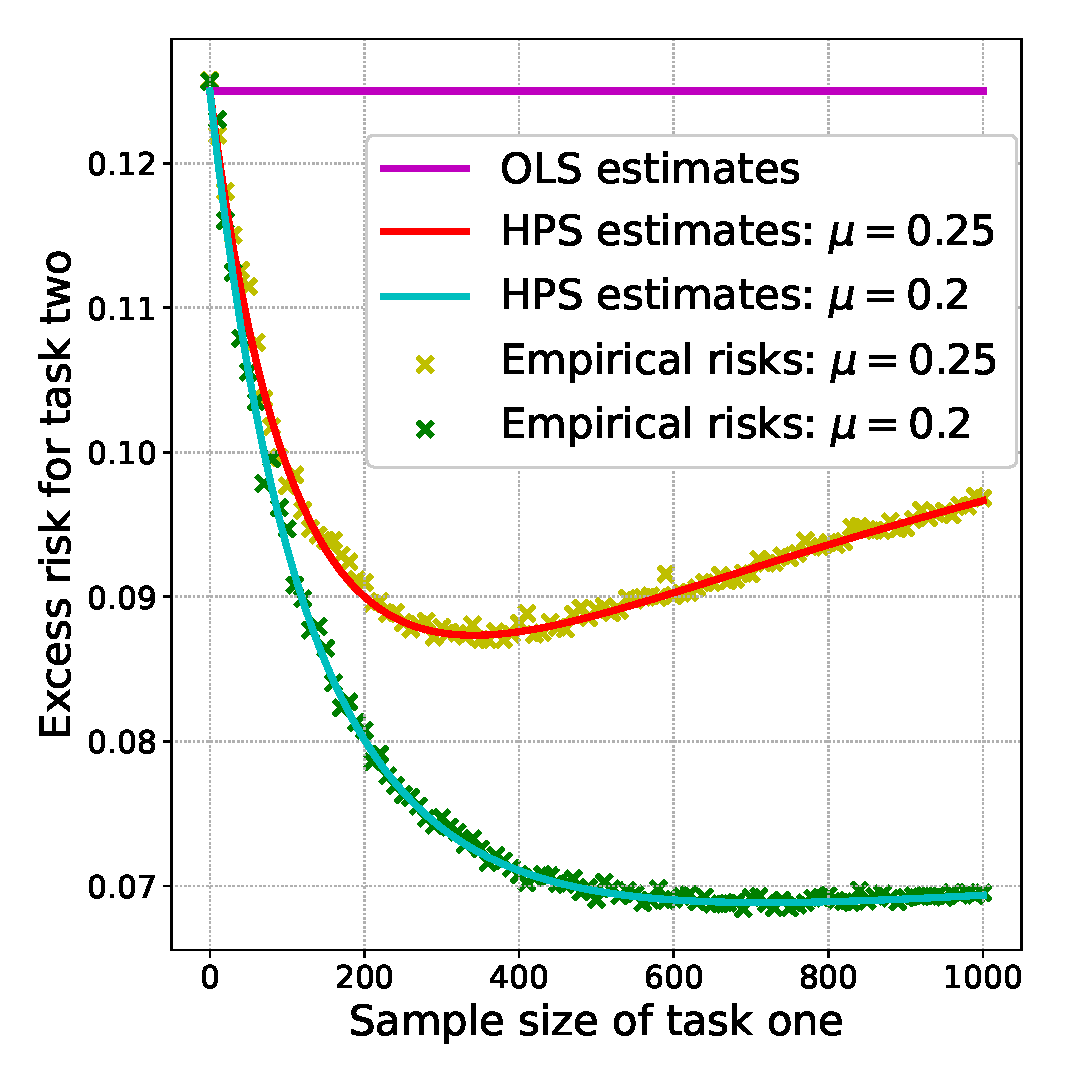
\includegraphics[width=0.95\textwidth]{figures/model_shift_positive.eps}
		\caption{Positive transfer}
		\label{fig_sec3_model_positive}
	\end{subfigure}\hfill%
	\begin{subfigure}[b]{0.33\textwidth}
		\centering
		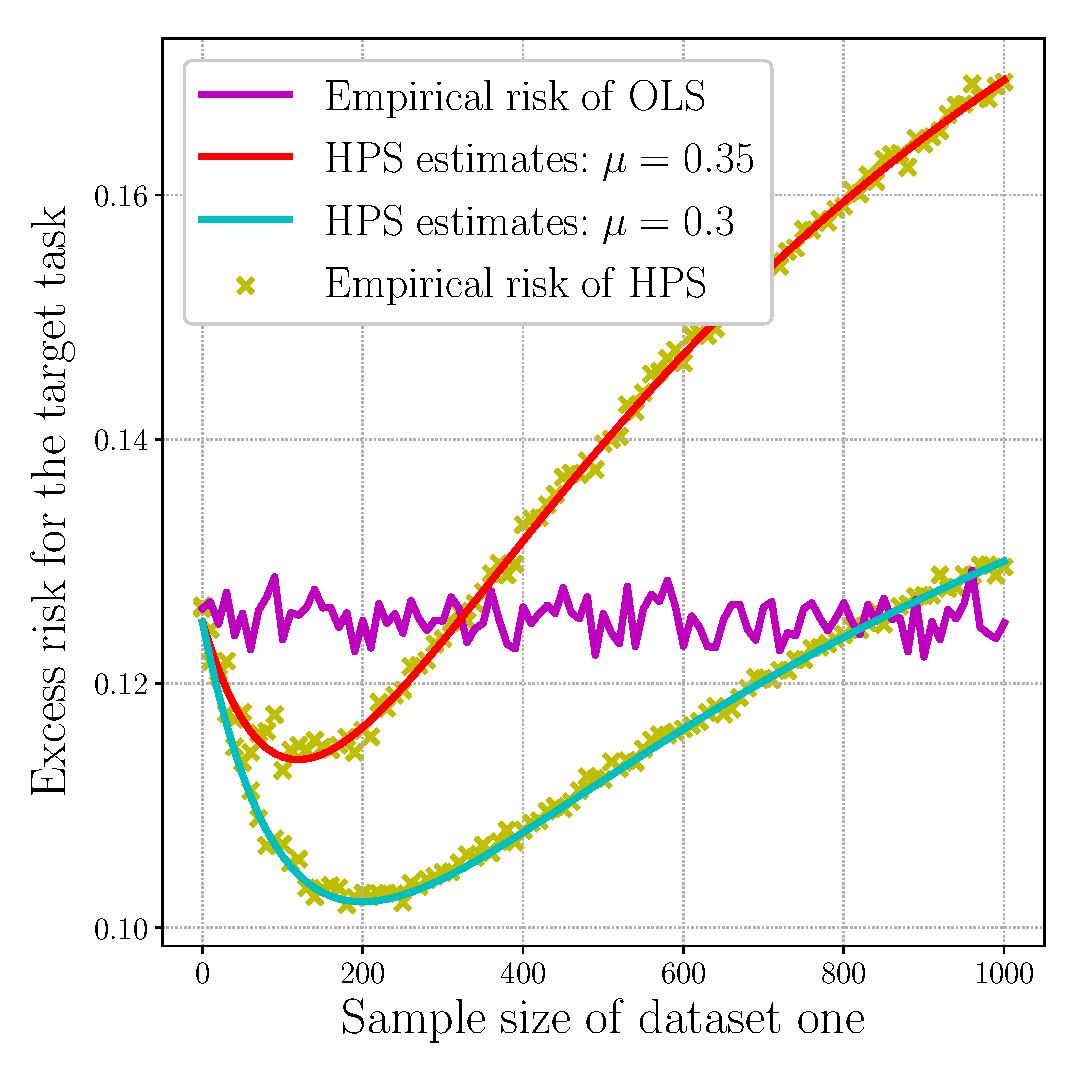
\includegraphics[width=0.95\textwidth]{figures/model_shift_transition.eps}
		\caption{From positive to negative transfer}
		\label{fig_sec3_model_transition}
	\end{subfigure}\hfill%
	\begin{subfigure}[b]{0.33\textwidth}
		\centering
		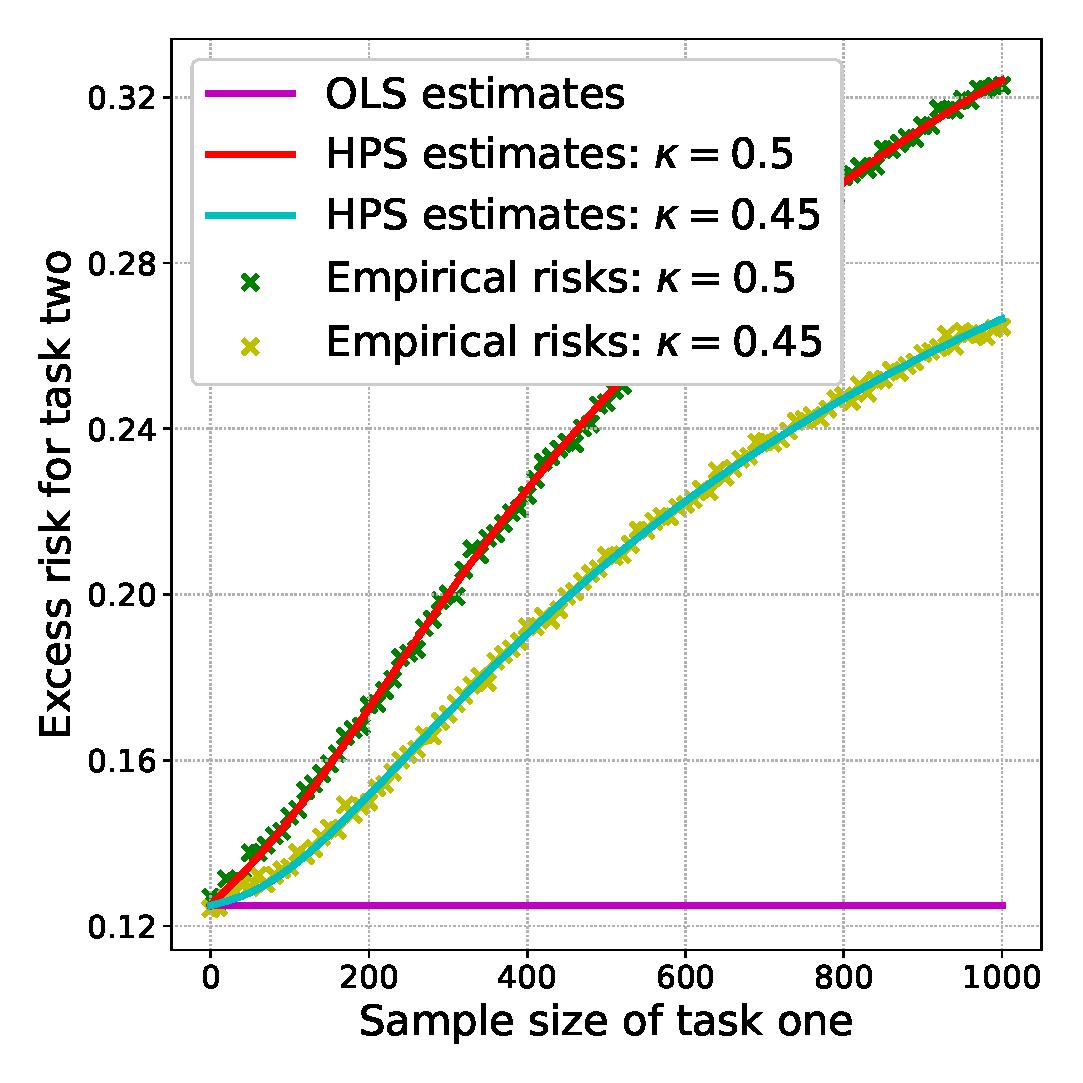
\includegraphics[width=0.95\textwidth]{figures/model_shift_negative.eps}
		\caption{Negative transfer}
		\label{fig_sec3_model_negative}
	\end{subfigure}	
	\caption{We illustrate three regimes of information transfer in HPS under model shift. When $\mu$ is small, HPS outperforms the OLS estimator irrespective of $n_1$. When $\mu$ is large, HPS performs worse than OLS. For an intermediate range of $\mu$, HPS outperforms OLS only for a restricted range of $n_1$. See Claim \ref{claim_model_shift} for the precise range of each regime. This simulation fixes $p = 100, n_2 = 300, \sigma = 1/2$ while varying $n_1, \mu$.}
	\label{fig_sec3_model_shift}
\end{figure}

\paragraph{Illustrative examples.}
While the estimates from Theorem \ref{cor_MTL_loss} are generally complex, we describe a simplified result for the random-effect model (cf. Section \ref{sec_data}).
Under the assumptions stated in Proposition \ref{lem_hat_v}, $\hat{a}$ is approximately equal to one.
Then, we can calculate that
\[ \cL_1(1) = \frac{p}{n_1 + n_2 - p} \text{ and } \cL_2(1) = \frac{n_1^2(n_1 + n_2 - p) + p n_1 n_2}{(n_1 + n_2)^2 (n_1 + n_2 - p)}, \text{ in which } \kappa(1) = \frac{n_2^2}{(n_1 + n_2)^2 - n_1 p}. \]
Thus, using that $\|\beta^{(1)}-\beta^{(2)}\|^2 = (2+\oo(1))\mu^2$ w.h.p., we conclude that for the random-effect model, the excess risk $L(\hat{\beta}_2^{\MTL}$ is approximately equal to
$$ g(n_1) \define \sigma^2 \cal L_1(1) +   2\mu^2 \cal L_2(1)= \frac{p\sigma^2}{n_1+n_2-p} +  2\mu^2 \cdot \frac{n_1^2 (n_1+n_2-p)+p n_1n_2}{(n_1+n_2)^2(n_1+n_2-p)}$$
plus lower order terms (that vanishes to zero as $p$ goes to infinity).
Next, we provide a detailed analysis of when combining task one using HPS transfers positively to task two, depending on sample sizes $n_1, n_2$, and model shift $\mu$.

\begin{claim}[Sample sizes vs. model shift]\label{claim_model_shift}
    Suppose Assumption \ref{assm_big1} and the random-effect model under equation \eqref{eq_re} and \eqref{para_rel} holds.
    Suppose further that $n_2 \ge 3p$.
    Then, there exists a large constant $C > 0$ such that the following holds w.h.p.,
    \begin{enumerate}
        \item[i)] If $\mu^2 \le \frac{\sigma^2 p}{2(n_2 - p)}$, then $L(\hat{\beta}_2^{\MTL}) \le L(\hat{\beta}_2^{\STL}) + \OO(p^{-C})$.
        \item[ii)] If $\frac{\sigma^2 p}{2(n_2 - p)} < \mu^2 < \frac{\sigma^2 n_2}{2(n_2 - p)}$, then there exists a deterministic constant $\rho$ such that if $n_1 \le \rho\cdot p$, then $L(\hat{\beta}_2^{\MTL}) \le L(\hat{\beta}_2^{\STL}) + \OO(p^{-C})$, else $L(\hat{\beta}_2^{\STL}) \le L(\hat{\beta}_2^{\MTL}) + \OO(p^{-C})$.
        \item[iii)] If $\frac{\sigma^2 n_2} {2(n_2 - p)} \le \mu^2$, then $L(\hat{\beta}_2^{\STL}) \le L(\hat{\beta}_2^{\MTL}) + \OO(p^{-C})$.
    \end{enumerate}
\end{claim}

\begin{proof}
By Theorem \ref{cor_MTL_loss} and the discussion above, we have that $L(\hat{\beta}_2^{\MTL}) = g(n) + \OO(p^{-C})$ w.h.p.
By Lemma \ref{fact_tr}, we have that the excess risk of the OLS estimator for task two satisfies
\begin{align*}
    L(\hat{\beta}_2^{\STL})
    = \sigma^2 \cdot \bigtr{\Sigma^{(2)}\Big((X^{(2)})^{\top} X^{(2)} \Big)^{-1}}
    = \frac{\sigma^2 p}{n_2 - p} + \OO(p^{-C}).
\end{align*}
Thus, whether or not $L(\hat{\beta}_2^{\MTL}) \le L(\hat{\beta}_2^{\STL})$ reduces to comparing $g(n_1)$ and $\frac{\sigma^2 p}{n_2 - p}$---let $h(n_1)$ be their difference.
We can write $h(n_1)$ as
\[ h(n_1) = 2\mu^2 \cdot \frac{n_1^2 (n_1 + n_2 - p) + p n_1 n_2}{(n_1 + n_2)^2 (n_1 + n_2 - p)} - \frac{\sigma^2 p n_1}{(n_1 + n_2 - p)(n_2 - p)}. \]
We observe that the sign of $h(n_1)$ is the same as the sign of the following simplified polynomial
\begin{align*}
    \tilde h(n_1) &= 2\mu^2 (n_2 - p) (n_1 (n_1 + n_2 - p) + p n_2) - \sigma^2 (n_1 + n_2)^2 \\
    &= \big(2\mu^2 (n_2 - p) - \sigma^2\big) n_1^2 + (2\mu^2 (n_2 - p)^2 - 2\sigma^2 p n_2) n_1 + \big(2\mu^2 (n_2 - p) p n_2 - \sigma^2 p n_2^2\big).
\end{align*}
Let $C_0, C_1, C_2$ be the coefficient of $n_1^0, n_1^1, n_1^2$ above, respectively.
We argue about each claim as follows.

For claim i), if $\mu^2 \le \frac{\sigma^2 p}{2(n_2 - p)}$, then $C_0, C_1, C_2$ are all at most zero.
Thus, $\tilde h(n_1) \le 0$, which implies that $h(n_1) \le 0$.

For claim ii), if $\frac{\sigma^2 p}{2(n_2 - p)}< \mu^2 < \frac{\sigma^2 n_2}{2(n_2 - p)}$ (recall that $n_2 > p$ by Assumption \ref{assm_big1}), then $C_2 > 0$ and $C_0 < 0$.
Thus, $\tilde{h}(n_1)$ has a positive root and a negative root.
Let $\rho$ be the positive root.
Hence, if $n_1 \le \rho \cdot p$, then $\tilde h(n_1) \le 0$.
Otherwise, $\tilde h(n_1) \ge 0$.

For claim iii), if $\frac{\sigma^2 n_2}{2(n_2 - p)} \le \mu^2$, then $C_1 \ge 0$ and $C_2 \ge 0$.
Furthermore, $\frac{\sigma^2 p n_2}{(n_2 - p)^2} \le \frac{\sigma^2 n_2}{2(n_2 - p)}$ because $n_2 \ge 3p$ by our assumption.
Thus, $C_2$ is non-negative as well, which implies $\tilde h(n_1) \ge 0$.
\end{proof}

As a remark, when $p < n_2 < 3p$, similar results can be derived using the above arguments (details omitted).
Figure \ref{fig_sec3_model_shift} illustrates Claim \ref{claim_model_shift} for different regimes of model shift.
First, we observe that our estimates accurately match with the empirical risks.
Second, as we vary the model shift parameter $\mu$, we observe the three information transfer regimes, as Claim \ref{claim_model_shift} suggests.





\subsection{Covariate and model shift}


For the bias limit, we have the following proposition.

\begin{theorem}[Bias estimates under covariate and model shift]\label{prop_main_RMT}
%The bias equation \eqref{Lbias} satisfies the following limit with high probability: Let $S$ be an arbitrary subset of the unit sphere in dimension $p$ whose size is polynomial in $p$, for any unit vector $w\in S$,
Under Assumption \ref{assm_big1}, for any small constant $c>0$ and large constant $C>0$, there exists a high probability event $\Xi$, on which the following estimate  holds for $L_{\bias}(a)$ in \eqref{Lbias}:
			\begin{align}
				& \bigabs{ L_{\bias}(a) -   (\beta^{(1)}- a\beta^{(2)} )^\top (\Sigma^{(1)})^{1/2} \Pi(a)(\Sigma^{(1)})^{1/2} (\beta^{(1)}- a\beta^{(2)})   }  \nonumber\\
				& \le \left[\left( 1+\sqrt{\frac{p}{n_1}}\right)^4 - 1 +\OO\left( n_1^{-1/2+2/\varphi + c}\right)\right] \frac{n_1^2 \lambda_1^2 \left\|(\Sigma^{(1)})^{1/2} \left(\beta^{(1)}- a\beta^{(2)}\right) \right\|^2}{  [(\sqrt{n_1}-\sqrt{p})^2 \lambda_p^2+ (\sqrt{n_2}-\sqrt{p})^2]^2}  \nonumber\\
				& + p^{-C} \left[\| \beta^{(1)}\|^2 + \| \beta^{(2)}\|^2 \right], \label{lem_cov_derv_eq}
			\end{align}
%			\begin{align}\label{lem_cov_derv_eq}
%				\bigabs{ L_{\bias}(a) - \left\|\frac{n_1}{n_1+n_2}  \frac{\left[a_3 M(a)^\top M(a) + (a_4 + 1) \right]^{1/2}}{ a_1 M(a)^\top M(a) + a_2 } M(a)^\top (\Sigma^{(1)})^{1/2} \left(\beta^{(1)}- a\beta^{(2)}\right)\right\|^2   } \le  \frac{p^{-c_{\varphi}}}{(n_1+n_2)^2},
%			\end{align}
				uniformly in all $a\in \R$. Here $\lambda_1$ and $\lambda_p$ are respectively the largest and smallest singular values of $M(a)$, $\Pi(a)$ is a $p\times p$ matrix defined as
				$$\Pi(a):=\frac{n_1^2}{(n_1+n_2)^2}  M(a)  \frac{a_3 M(a)^\top M(a) + (a_4 + 1) }{[a_1 M(a)^\top M(a) + a_2 ]^2} M(a)^\top  ,$$
				 and $(a_{3},a_4)$ is the solution of the following system of equations % with $b_k = \frac1{p}\sum_{i=1}^p \frac{\lambda_i^{2k}} {(\lambda_i^2 a_1 + a_2)^2}$, for $k = 0, 1, 2$:
		\be  \label{eq_a34extra}
		\begin{split}
				& a_3 + a_4 = \frac{1}{n_1 + n_2}\sum_{i=1}^p \frac{1}{\lambda_i^2 a_1 + a_2}, \\
				& a_3 + \frac{1}{n_1 + n_2} \sum_{i=1}^p \frac{\lambda_i^2 (a_2 a_3-a_1 a_4 )}{(\lambda_i^2 a_1 + a_2)^2} = \frac{1}{n_1 + n_2} \sum_{i=1}^p \frac{\lambda_i^2 a_1}{(\lambda_i^2 a_1 + a_2)^{2}},
%				\left(\frac{\rho_1}{a_1^{2}} -  b_2  \right)\cdot  a_3 -  b_1 \cdot  a_4 = b_1,\quad \left(\frac{\rho_2}{a_2^{2}}-  b_0\right)\cdot  a_4 - b_1 \cdot  a_3
%				= b_0.
			\end{split}
			\ee
			where we recall that $(a_1,a_2)$ is the solution of \eqref{eq_a12extra}.
\end{theorem}

Note that the first error term on the right-hand side of \eqref{lem_cov_derv_eq} is typically smaller than the main term $ (\beta^{(1)}- a\beta^{(2)} )^\top (\Sigma^{(1)})^{1/2} \Pi(a)(\Sigma^{(1)})^{1/2} (\beta^{(1)}- a\beta^{(2)})  $ by a factor of $\OO(\sqrt{p/n_1} + n_1^{-1/2+2/\varphi + c})$. Hence \eqref{lem_cov_derv_eq} only gives an exact asymptotic limit in the regime $n_1\gg p$. Moreover, by equations \eqref{eq_a12extra} and \eqref{eq_a34extra} we have
$$a_1 =\frac{n_1}{n_1+n_2} + \OO\left( \frac{p}{n_1+n_2}\right), \quad a_3 =\frac{n_3}{n_1+n_2} + \OO\left( \frac{p}{n_1+n_2}\right),$$
and
$$a_3 =\OO\left( \frac{p}{n_1+n_2}\right),\quad a_4 =\OO\left( \frac{p}{n_1+n_2}\right).$$
Using these estimates, it is easy to check that
\begin{align}
& (\beta^{(1)}- a\beta^{(2)} )^\top (\Sigma^{(1)})^{1/2} \Pi(a)(\Sigma^{(1)})^{1/2} (\beta^{(1)}- a\beta^{(2)})   \nonumber \\
&=\left\| (\Sigma^{(2)})^{1/2}\frac{1}{a^2\Sigma^{(1)}+\Sigma^{(2)}} a \Sigma^{(1)} \left(\beta^{(1)}- a\beta^{(2)}\right) \right\|^2 + \OO\left( \frac{p\left\|\beta^{(1)}- a\beta^{(2)}\right\|^2}{n_1+n_2}  \right)  . \label{bias_LLN}
\end{align}
Hence \eqref{lem_cov_derv_eq} is consistent with the result obtained by replacing $ (X^{(1)})^\top X^{(1)}$ and $ (X^{(2)})^\top X^{(2)}$ with $n_1\Sigma^{(1)}$ and $n_2\Sigma^{(2)}$, respectively, in $L_{\bias} (a) $ using the law of large numbers in the regime $n_1\gg p$. However, simulations show that our estimate \eqref{lem_cov_derv_eq} is more precise than the first term on the right-hand side of \eqref{bias_LLN}.

\begin{remark}
%First, our result in Corollary \ref{cor_MTL_loss} involves an error term that scales down with $n_1$.
%Tightening this error bound requires showing the limit of $\normFro{({Z^{(1)}}^{\top} Z^{(1)} + {Z^{(2)}}^{\top} Z^{(2)})^{-1} {Z^{(1)}}^{\top} Z^{(1)}}^2$ for two isotropic sample covariance matrices.
%This requires studying the asymptotic singular values distribution of the non-symmetric matrix $({Z^{(1)}}^{\top} Z^{(1)})^{-1}{Z^{(2)}}^{\top} Z^{(2)}+\id$, which is still an open problem in random matrix theory.
%\begin{remark}
The main error in Proposition \ref{prop_main_RMT} comes from approximating $(Z^{(1)})^\top Z^{(1)}$ by $n_1\id_{n_1\times n_2}$ using Corollary \ref{fact_minv} in the supplement \cite{MTL_suppl}. In order to improve this estimate and obtain an exact asymptotic result, one needs to study the singular value distribution of the  random matrix $\cal X + a^2$ for any fixed $a\in \R$, where $\cal X:=[(X^{(1)})^{\top}X^{(1)}]^{-1}(X^{(2)})^{\top}X^{(2)}$. We remark that the eigenvalues of $\cal X$ have been studied in the name of Fisher matrices \cite{Fmatrix}. However, since $\cal X$ is not symmetric, its singular values are different from its eigenvalues. To the best of our knowledge, the asymptotic singular value behavior of $\cal X$ is still an open problem in random matrix theory, and the study of the singular values of $\cal X + a^2$ will be even harder. We leave this problem to future study.

We also remark for the general case with covariate shift, the method in Section \ref{sec_sizeratio} for the bias term also fails, because we cannot reduce the problem into the free addition of two random matrices that are asymptotically freely independent.
%\end{remark}
\end{remark}